\section{Thu thập và Phân tích Dữ liệu}
\label{sec:data}

\subsection{Nguồn và Phương pháp Thu thập}

Bộ dữ liệu của đồ án được xây dựng cho bài toán phát hiện đối tượng với ba lớp: \texttt{motorbike}, \texttt{helmet} và \texttt{non-helmet}. Nhóm sử dụng kết hợp dữ liệu công khai, dữ liệu tự thu thập từ video giao thông và nhãn bán tự động để tăng độ đa dạng về bối cảnh đường phố, góc camera và mật độ phương tiện.

Các nguồn dữ liệu chính được tóm tắt trong Bảng~\ref{tab:data-sources}. Những bộ dữ liệu dạng COCO/Roboflow cung cấp nhãn ban đầu cho xe máy và mũ bảo hiểm. Bên cạnh đó, nhóm thu thập thêm video giao thông từ YouTube bằng \texttt{yt-dlp}, trích xuất khung hình bằng OpenCV, sau đó dùng Ollama LLaVA để lọc sơ bộ các ảnh có khả năng chứa người không đội mũ bảo hiểm. Với phần dữ liệu còn thiếu nhãn hoặc nhãn chưa đầy đủ, Grounding DINO được dùng để sinh pseudo-label, rồi nhóm kiểm tra và hiệu chỉnh thủ công bằng CVAT.

\begin{table}[H]
    \centering
    \small
    \caption{Nguồn dữ liệu và vai trò trong quá trình xây dựng bộ dữ liệu}
    \label{tab:data-sources}
    \begin{tabularx}{\textwidth}{l l X}
        \toprule
        \textbf{Nguồn} & \textbf{Dạng dữ liệu} & \textbf{Vai trò} \\
        \midrule
        Các bộ COCO/Roboflow & Ảnh và annotation COCO & Cung cấp nhãn ban đầu cho \texttt{motorbike}, \texttt{helmet} và một phần \texttt{non-helmet}. \\
        Video giao thông YouTube & Video, frame trích xuất & Bổ sung bối cảnh giao thông Việt Nam, nhiều góc nhìn camera và mật độ xe khác nhau. \\
        Ollama LLaVA & Bộ lọc ảnh & Lọc nhanh các frame có dấu hiệu người không đội mũ để giảm khối lượng gán nhãn thủ công. \\
        Grounding DINO và CVAT & Pseudo-label và hiệu chỉnh thủ công & Sinh nhãn đề xuất, sau đó kiểm tra, sửa bbox và hợp nhất lại vào các file COCO. \\
        \bottomrule
    \end{tabularx}
\end{table}

Dựa trên notebook EDA, Hình~\ref{fig:eda-source-contribution} cho thấy dữ liệu được đóng góp từ nhiều nguồn khác nhau. Hai bộ dữ liệu \texttt{CS114\_helmet\_detection\_Final.v1i.coco} và \texttt{Motobike Detection.v1i.coco} đóng góp nhiều ảnh train/test, trong khi nguồn \texttt{grounding\_dino\_no\_helmet} bổ sung thêm các ảnh giàu trường hợp vi phạm sau bước sinh nhãn và kiểm tra lại. Sau khi chốt dữ liệu, validation và test được giữ cố định cho đánh giá; tập train sử dụng file \texttt{instances\_train\_merged.json} để tăng độ phủ nhãn. Cách kết hợp này giúp bộ dữ liệu không phụ thuộc vào một nguồn duy nhất, dù vẫn cần chú ý khác biệt phân phối giữa các nguồn.

\begin{figure}[H]
    \centering
    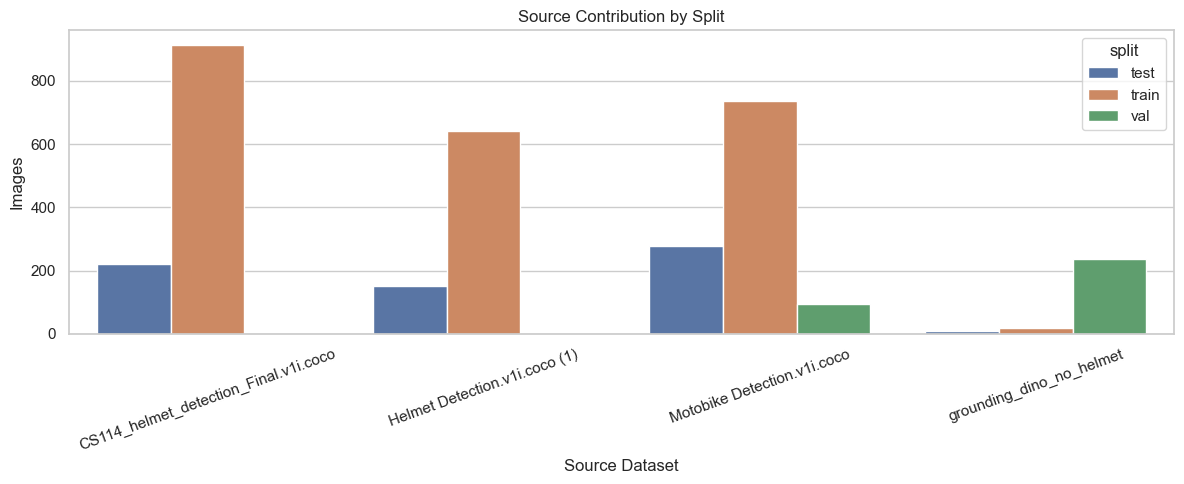
\includegraphics[width=0.92\textwidth]{img/eda/source_contribution.png}
    \caption{Đóng góp số lượng ảnh của từng nguồn dữ liệu theo train/validation/test.}
    \label{fig:eda-source-contribution}
\end{figure}

Dữ liệu cuối cùng được lưu theo định dạng COCO JSON, trong đó mỗi annotation chứa \texttt{image\_id}, \texttt{category\_id}, bounding box dạng \texttt{[x, y, w, h]}, diện tích bbox và cờ \texttt{iscrowd}. Ảnh được chuẩn hóa về kích thước 640x640 bằng letterbox với padding xám, giúp các mô hình YOLO, RT-DETR và Faster R-CNN dùng cùng một đầu vào. Cấu trúc lưu trữ gồm ba thư mục ảnh \texttt{train}, \texttt{val}, \texttt{test} và các file annotation tương ứng trong thư mục \texttt{annotations}.

\subsection{Tiền xử lý và Làm sạch}

Quy trình tiền xử lý được hiện thực trong các script ở thư mục \texttt{crawl/scripts}. Trước hết, nhãn từ nhiều nguồn được ánh xạ về ba lớp thống nhất. Các nhãn ngoài phạm vi bài toán như \texttt{person}, \texttt{rider} hoặc các lớp không liên quan bị loại bỏ để tránh làm nhiễu detector. Những biến thể tên lớp như \textit{motorcycle}, \textit{scooter}, \textit{no helmet} hoặc \textit{without helmet} được chuẩn hóa về tên lớp chính thức.

Sau bước chuẩn hóa nhãn, hệ thống kiểm tra sự tồn tại của ảnh, khả năng đọc ảnh, kích thước ảnh và tính hợp lệ của bbox. Các bbox có chiều rộng hoặc chiều cao nhỏ hơn hoặc bằng 1 pixel bị loại bỏ; bbox vượt biên ảnh được cắt về đúng kích thước ảnh. Những ảnh không còn đối tượng hợp lệ sau bước lọc cũng không được đưa vào tập dữ liệu cuối.

Để giảm trùng lặp, nhóm dùng hai mức kiểm tra. Trùng lặp chính xác được phát hiện bằng MD5 của file ảnh; các ảnh gần trùng được phát hiện bằng average hash với ngưỡng Hamming nhỏ. Với dữ liệu lấy từ video, nhiều frame liên tiếp thường gần giống nhau; nếu đưa đồng thời vào train và test, kết quả đánh giá có thể bị lạc quan. Vì vậy, script tạo khóa nhóm theo video, mốc thời gian hoặc mẫu tên file, sau đó chia train/validation/test theo nhóm thay vì chia ngẫu nhiên từng ảnh riêng lẻ.

Bảng~\ref{tab:data-cleaning-steps} tóm tắt các vấn đề chất lượng dữ liệu chính và cách xử lý.

\begin{table}[H]
    \centering
    \small
    \caption{Các bước làm sạch và kiểm soát chất lượng dữ liệu}
    \label{tab:data-cleaning-steps}
    \begin{tabularx}{\textwidth}{l X X}
        \toprule
        \textbf{Vấn đề} & \textbf{Ảnh hưởng} & \textbf{Cách xử lý} \\
        \midrule
        Tên lớp không thống nhất & Mô hình học nhiều lớp trùng nghĩa hoặc sai mục tiêu & Chuẩn hóa tất cả nhãn về ba lớp \texttt{motorbike}, \texttt{helmet}, \texttt{non-helmet}. \\
        Bbox sai hoặc vượt biên ảnh & Gây lỗi khi huấn luyện và làm sai loss định vị & Cắt bbox theo biên ảnh, loại bbox quá nhỏ hoặc không hợp lệ. \\
        Ảnh thiếu file hoặc không đọc được & Pipeline huấn luyện bị dừng giữa chừng & Kiểm tra đường dẫn ảnh, loại ảnh thiếu hoặc hỏng. \\
        Frame gần trùng từ cùng video & Rò rỉ dữ liệu giữa train và test & Khử trùng lặp bằng MD5/average hash và chia dữ liệu theo nhóm. \\
        Nhãn tự động chưa chính xác & Tạo nhiễu cho tập huấn luyện & Dùng CVAT để kiểm tra, sửa bbox và chỉ giữ val/test ở dạng nhãn gốc đã kiểm duyệt. \\
        \bottomrule
    \end{tabularx}
\end{table}

Tập train sử dụng file \texttt{instances\_train\_merged.json}, tức là nhãn thủ công được gộp thêm pseudo-label để giảm tình trạng thiếu nhãn ở một số lớp. Ngược lại, validation và test không được gộp pseudo-label sau cùng; hai tập này được giữ ổn định để đánh giá khách quan khả năng tổng quát hóa.

\subsection{Phân tích Khám phá Dữ liệu (EDA)}

Sau khi làm sạch, bộ dữ liệu cuối gồm 3,298 ảnh và 14,797 annotation. Tỷ lệ chia dữ liệu được giữ gần 70/10/20 theo số ảnh, tương ứng train, validation và test. Bảng~\ref{tab:data-split-eda} cho thấy tập train chiếm phần lớn ảnh để phục vụ huấn luyện, trong khi test có 659 ảnh để đánh giá cuối.

\begin{table}[H]
    \centering
    \small
    \caption{Thống kê tổng quan theo từng tập dữ liệu}
    \label{tab:data-split-eda}
    \begin{tabular}{lrrrr}
        \toprule
        \textbf{Tập} & \textbf{Số ảnh} & \textbf{Tỷ lệ ảnh} & \textbf{Số annotation} & \textbf{Annotation/ảnh} \\
        \midrule
        Train & 2309 & 70.0\% & 11047 & 4.78 \\
        Validation & 330 & 10.0\% & 1889 & 5.72 \\
        Test & 659 & 20.0\% & 1861 & 2.82 \\
        \midrule
        Tổng & 3298 & 100.0\% & 14797 & 4.49 \\
        \bottomrule
    \end{tabular}
\end{table}

Phân bố nhãn theo lớp được trình bày trong Bảng~\ref{tab:class-distribution-eda} và Hình~\ref{fig:eda-class-distribution}. Lớp \texttt{helmet} chiếm tỷ lệ lớn nhất với 8,445 bbox, tương đương 57.1\% tổng số annotation. Lớp \texttt{non-helmet} chỉ có 1,571 bbox, tương đương 10.6\%. Đây là đặc điểm quan trọng của bài toán: vi phạm không đội mũ thường ít hơn nhiều so với các trường hợp đội mũ, nhưng lại là lớp quan trọng nhất đối với hệ thống cảnh báo.

\begin{table}[H]
    \centering
    \small
    \caption{Phân bố annotation theo lớp và theo tập dữ liệu}
    \label{tab:class-distribution-eda}
    \begin{tabular}{lrrrrr}
        \toprule
        \textbf{Lớp} & \textbf{Train} & \textbf{Validation} & \textbf{Test} & \textbf{Tổng} & \textbf{Tỷ lệ} \\
        \midrule
        \texttt{motorbike} & 3408 & 906 & 467 & 4781 & 32.3\% \\
        \texttt{helmet} & 6739 & 450 & 1256 & 8445 & 57.1\% \\
        \texttt{non-helmet} & 900 & 533 & 138 & 1571 & 10.6\% \\
        \midrule
        Tổng & 11047 & 1889 & 1861 & 14797 & 100.0\% \\
        \bottomrule
    \end{tabular}
\end{table}

\begin{figure}[H]
    \centering
    
\includegraphics[width=0.92\textwidth]{img/eda/class_distribution.png}
    \caption{Phân bố số lượng và tỷ lệ annotation của từng lớp theo từng tập dữ liệu.}
    \label{fig:eda-class-distribution}
\end{figure}

Từ các thống kê trên, nhóm rút ra ba nhận xét chính. Thứ nhất, dữ liệu có mật độ annotation tương đối cao, đặc biệt ở tập train và validation, phản ánh đặc thù ảnh giao thông có nhiều xe và người trong cùng khung hình. Thứ hai, phân bố lớp bị mất cân bằng: \texttt{helmet} xuất hiện nhiều hơn \texttt{non-helmet} khoảng 5.4 lần. Điều này làm mô hình dễ thiên về lớp phổ biến và có thể bỏ sót vi phạm nhỏ hoặc mờ. Thứ ba, kích thước đối tượng không đồng đều: bbox xe máy thường lớn hơn nhiều so với vùng đầu/mũ, trong khi \texttt{helmet} và \texttt{non-helmet} thường nhỏ, bị che khuất hoặc nằm xa camera.

Hình~\ref{fig:eda-bbox-density} minh họa thêm các đặc điểm hình học của annotation. Phần lớn ảnh có số đối tượng thấp đến trung bình, nhưng vẫn có một số ảnh đông phương tiện với nhiều bbox trong cùng khung hình. Phân bố diện tích bbox cho thấy \texttt{motorbike} thường có diện tích lớn hơn rõ rệt, còn \texttt{helmet} và \texttt{non-helmet} tập trung ở vùng diện tích nhỏ hơn. Đây là một trong các nguyên nhân làm bài toán khó: mô hình phải phát hiện đồng thời xe máy lớn và vùng đầu/mũ nhỏ trong ảnh giao thông.

\begin{figure}[H]
    \centering
    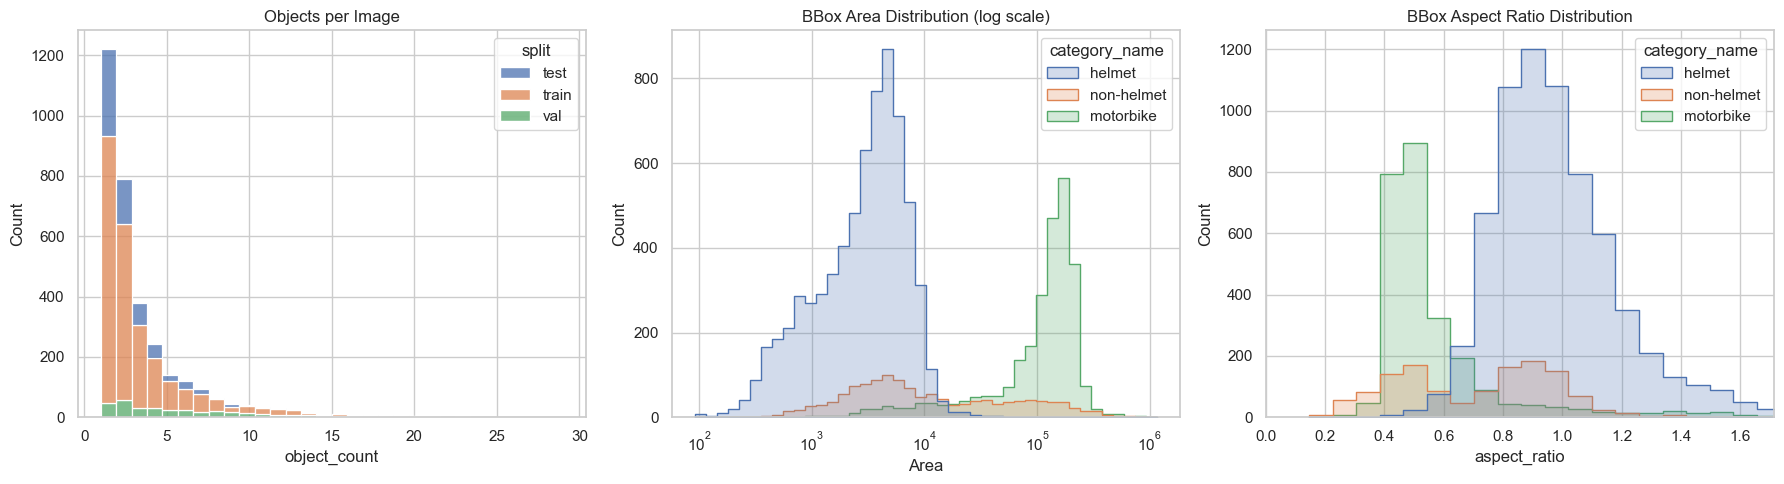
\includegraphics[width=0.96\textwidth]{img/eda/bbox_and_density_metrics.png}
    \caption{Phân bố số đối tượng trên mỗi ảnh, diện tích bbox và tỷ lệ cạnh bbox theo lớp.}
    \label{fig:eda-bbox-density}
\end{figure}

Các vấn đề trên ảnh hưởng trực tiếp đến lựa chọn mô hình và cách đánh giá. Vì lớp \texttt{non-helmet} là lớp hiếm nhưng quan trọng, nhóm không chỉ theo dõi mAP mà còn xem recall/AR và F1-score ở Chương~\ref{sec:results}. Ngoài ra, việc giữ test set độc lập và không dùng test trong quá trình chọn siêu tham số giúp hạn chế nguy cơ đánh giá quá lạc quan trên dữ liệu đã bị rò rỉ hoặc đã được tinh chỉnh gián tiếp.
